% Figure blocks for the six supplied figures (figures/ directory of the task; only these may be
% referenced). Each block is self-contained; place it where indicated in exhibits/README.md.
% Requires \usepackage{graphicx}. Labels referenced here that the report must define:
%   sec:method (Methodology), alg:cover (cover-encoding search, presented as Algorithm 1 because
%   figure_4.png prints "Algorithm 1"), def:valid (definition of valid/invalid encodings).
% Citation keys used: bavarian2022fim, dagan2024tokenizer, athiwaratkun2024alignment

% --- Figure: overview (Introduction) ---
\begin{figure}[t]
\begin{center}
% trim removes a stray rule and blank band at the top of the supplied PNG (1 px = 1 bp)
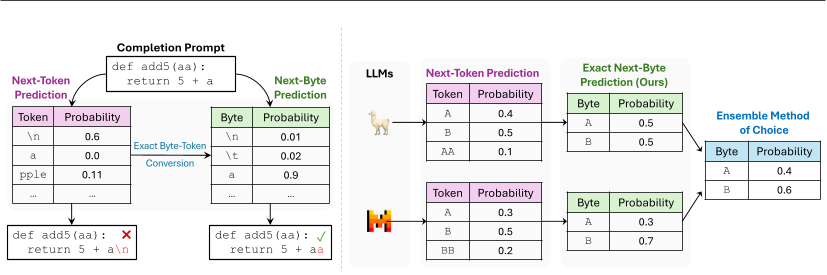
\includegraphics[width=\linewidth,trim={0 0 0 40},clip]{figures/figure_1.png}
\end{center}
\caption{Left: when a prompt ends mid-token, as in this schematic code completion example, a
tokenized LM suffers from tokenization bias: the correct continuation \texttt{a} (completing the
argument name \texttt{aa}) receives zero next-token probability. Converting the same model's
next-token predictions into exact next-byte predictions assigns it high probability. Right:
mapping the next-token predictions of LMs with different vocabularies to statistically equivalent
next-byte predictions (Section~\ref{sec:method}) puts them in a common space, where any ensemble
method, such as averaging or a mixture of experts, can be applied.}
\label{fig:overview}
\end{figure}

% --- Figure: tokenization bias, 1st-order Markov chain (problem setup / Section on bias) ---
\begin{figure}[t]
\begin{center}
% trim removes a stray rule at the top of the supplied PNG
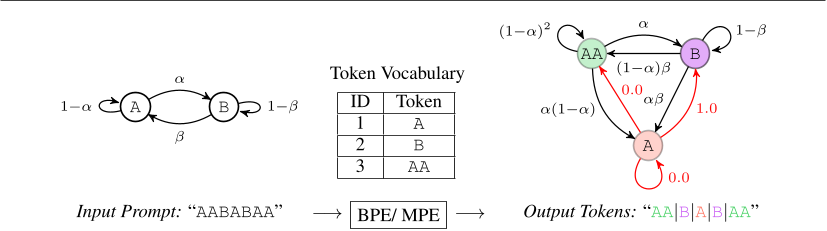
\includegraphics[width=\linewidth,trim={0 0 0 18},clip]{figures/figure_2.png}
\end{center}
\caption{Tokenization bias on a first-order Markov chain over the bytes \texttt{A} and
\texttt{B} (left), tokenized with the vocabulary \{\texttt{A}, \texttt{B}, \texttt{AA}\} by
BPE or MPE (middle). Because two consecutive \texttt{A} bytes are always merged into the token
\texttt{AA}, a standalone token \texttt{A} is always followed by \texttt{B} in encoded text.
Given the context token \texttt{A}, the tokenized model therefore assigns probability 0 to the
next token being \texttt{A} or \texttt{AA} and probability 1 to \texttt{B} (red edges, right),
whereas in the original chain the byte after \texttt{A} is \texttt{A} with probability
$1-\alpha$. This occurs whenever a prompt ends with a token that is a prefix of another token,
as is common in fill-in-the-middle (FIM) tasks.}
\label{fig:markov1}
\end{figure}

% --- Figure: tokenization bias and its correction, 3rd-order Markov chain (Experiments) ---
% Caption below the image (ICLR figure rule), as settled with paper-repo in paper-repo#4.
\begin{figure}[t]
\begin{center}
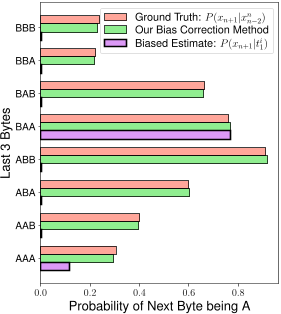
\includegraphics[width=0.33\linewidth]{figures/figure_3.png}
\end{center}
\caption{Tokenization bias and its correction on a third-order Markov chain. For each context
of the last three bytes, bars give the probability that the next byte is \texttt{A}: ground
truth $P(x_{n+1} \mid x_{n-2}^{n})$ of the chain (red), the estimate obtained by conditioning a
trained tokenized LM on its token history, $P(x_{n+1} \mid t_1^{k})$ (purple), and the
byte-level probability from our byte-token conversion applied to the same model
(Section~\ref{sec:method}; green). The token-conditioned estimate is close to zero for six of the
eight contexts, whereas the converted probabilities recover the ground truth.}
\label{fig:markov3}
\end{figure}

% --- Figure: cover encodings and Algorithm 1 (Methodology) ---
\begin{figure}[t]
\begin{center}
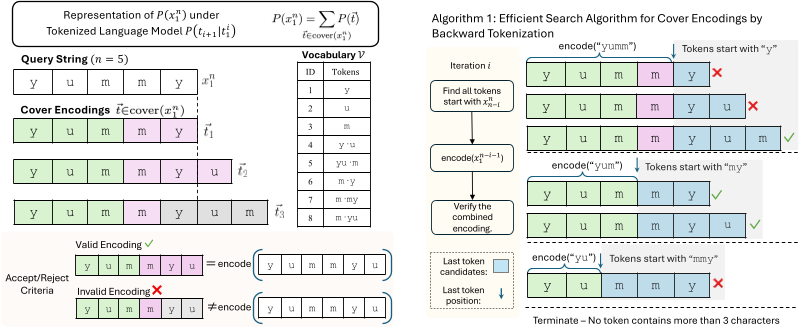
\includegraphics[width=\linewidth]{figures/figure_4.png}
\end{center}
\caption{Left: the probability $P(x_1^n)$ of a byte string under a tokenized LM is the sum of the
probabilities $P(\vec{t})$ of its cover encodings $\vec{t} \in \mathrm{cover}(x_1^n)$, shown for
the query string \texttt{yummy} ($n=5$) and an eight-token vocabulary. An encoding is valid if
re-encoding the bytes it decodes to returns the same tokens, and invalid otherwise
(Definition~\ref{def:valid}). Right: Algorithm~\ref{alg:cover} finds them by backward tokenization: at iteration $i$ it
lists the tokens that start with the last $i$ bytes, encodes the remaining prefix, and keeps the
combined encoding only if it is valid (green tick; red cross: invalid). The figure counts
iterations from zero. The search stops once the suffix is longer than every token (here, three
characters). The example uses BPE.}
\label{fig:cover}
\end{figure}

% --- Figure: next-byte sampling (Methodology, after Algorithm 1) ---
\begin{figure}[t]
\begin{center}
% trim removes a stray rule at the top of the supplied PNG
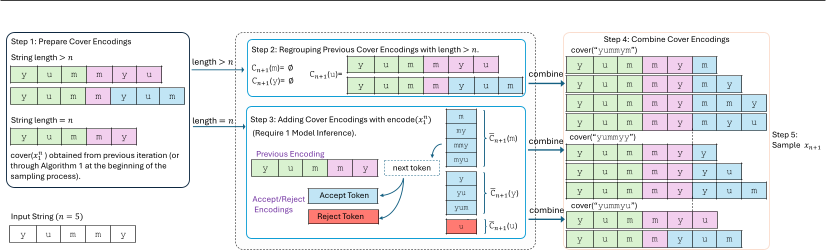
\includegraphics[width=\linewidth,trim={0 0 0 28},clip]{figures/figure_5.png}
\end{center}
\caption{Sampling the next byte $x_{n+1}$ from a tokenized LM $P(t_{k+1} \mid t_1^{k})$,
continuing the example of Figure~\ref{fig:cover}. Step~1: the cover encodings of $x_1^n$ come
from the previous iteration (or from Algorithm~\ref{alg:cover} at the start) and are split by
the length of the string they decode to. Step~2: encodings longer than $n$ bytes are regrouped
by their $(n{+}1)$-th byte. Step~3: encodings of exactly $n$ bytes are extended by next tokens
predicted from $\mathrm{encode}(x_1^n)$ (one model call), and each candidate is accepted or
rejected by the validity criterion. Step~4: both groups are combined into the cover encodings of
each candidate string $x_1^n x_{n+1}$. Step~5: $x_{n+1}$ is sampled from the resulting byte-level
distribution. The probabilities $P(\vec{t})$ are omitted for clarity.}
\label{fig:sampling}
\end{figure}

% --- Figure: FIM results (Experiments). Contains log Table 1; no separate table needed. ---
\begin{figure}[t]
\begin{center}
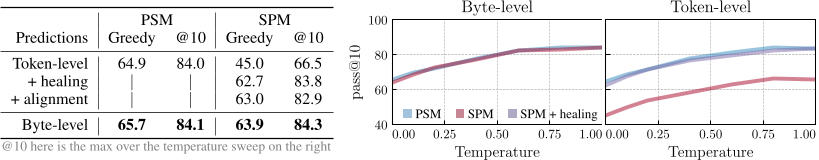
\includegraphics[width=\linewidth]{figures/figure_6.png}
\end{center}
\caption{Pass rates (\%) on the HumanEval Random Span infilling benchmark
\citep{bavarian2022fim} with CodeLlama-7b, using the Prefix-Suffix-Middle (PSM) and
Suffix-Prefix-Middle (SPM) prompt templates. Left: greedy pass rate and pass@10, where @10 is the
maximum over the temperature sweep on the right. The baselines token healing
\citep{dagan2024tokenizer} and token alignment \citep{athiwaratkun2024alignment} target prompts that
end mid-token and are evaluated in SPM only (vertical bars). Right: pass@10 versus sampling
temperature for byte-level and token-level predictions (the token-level panel also shows SPM with
token healing). SPM forces predictions from the middle of
a token: token-level greedy drops from 64.9 (PSM) to 45.0 (SPM), while byte-level predictions
reach 63.9 in SPM, above both baselines, and are highest in every column.}
\label{fig:fim}
\end{figure}
